\chapter{Related Work}
\setcounter{section}{0}

\section{Background}

\section{Indico}


\subsection{Events}

\begin{figure}[H]
    \centering
    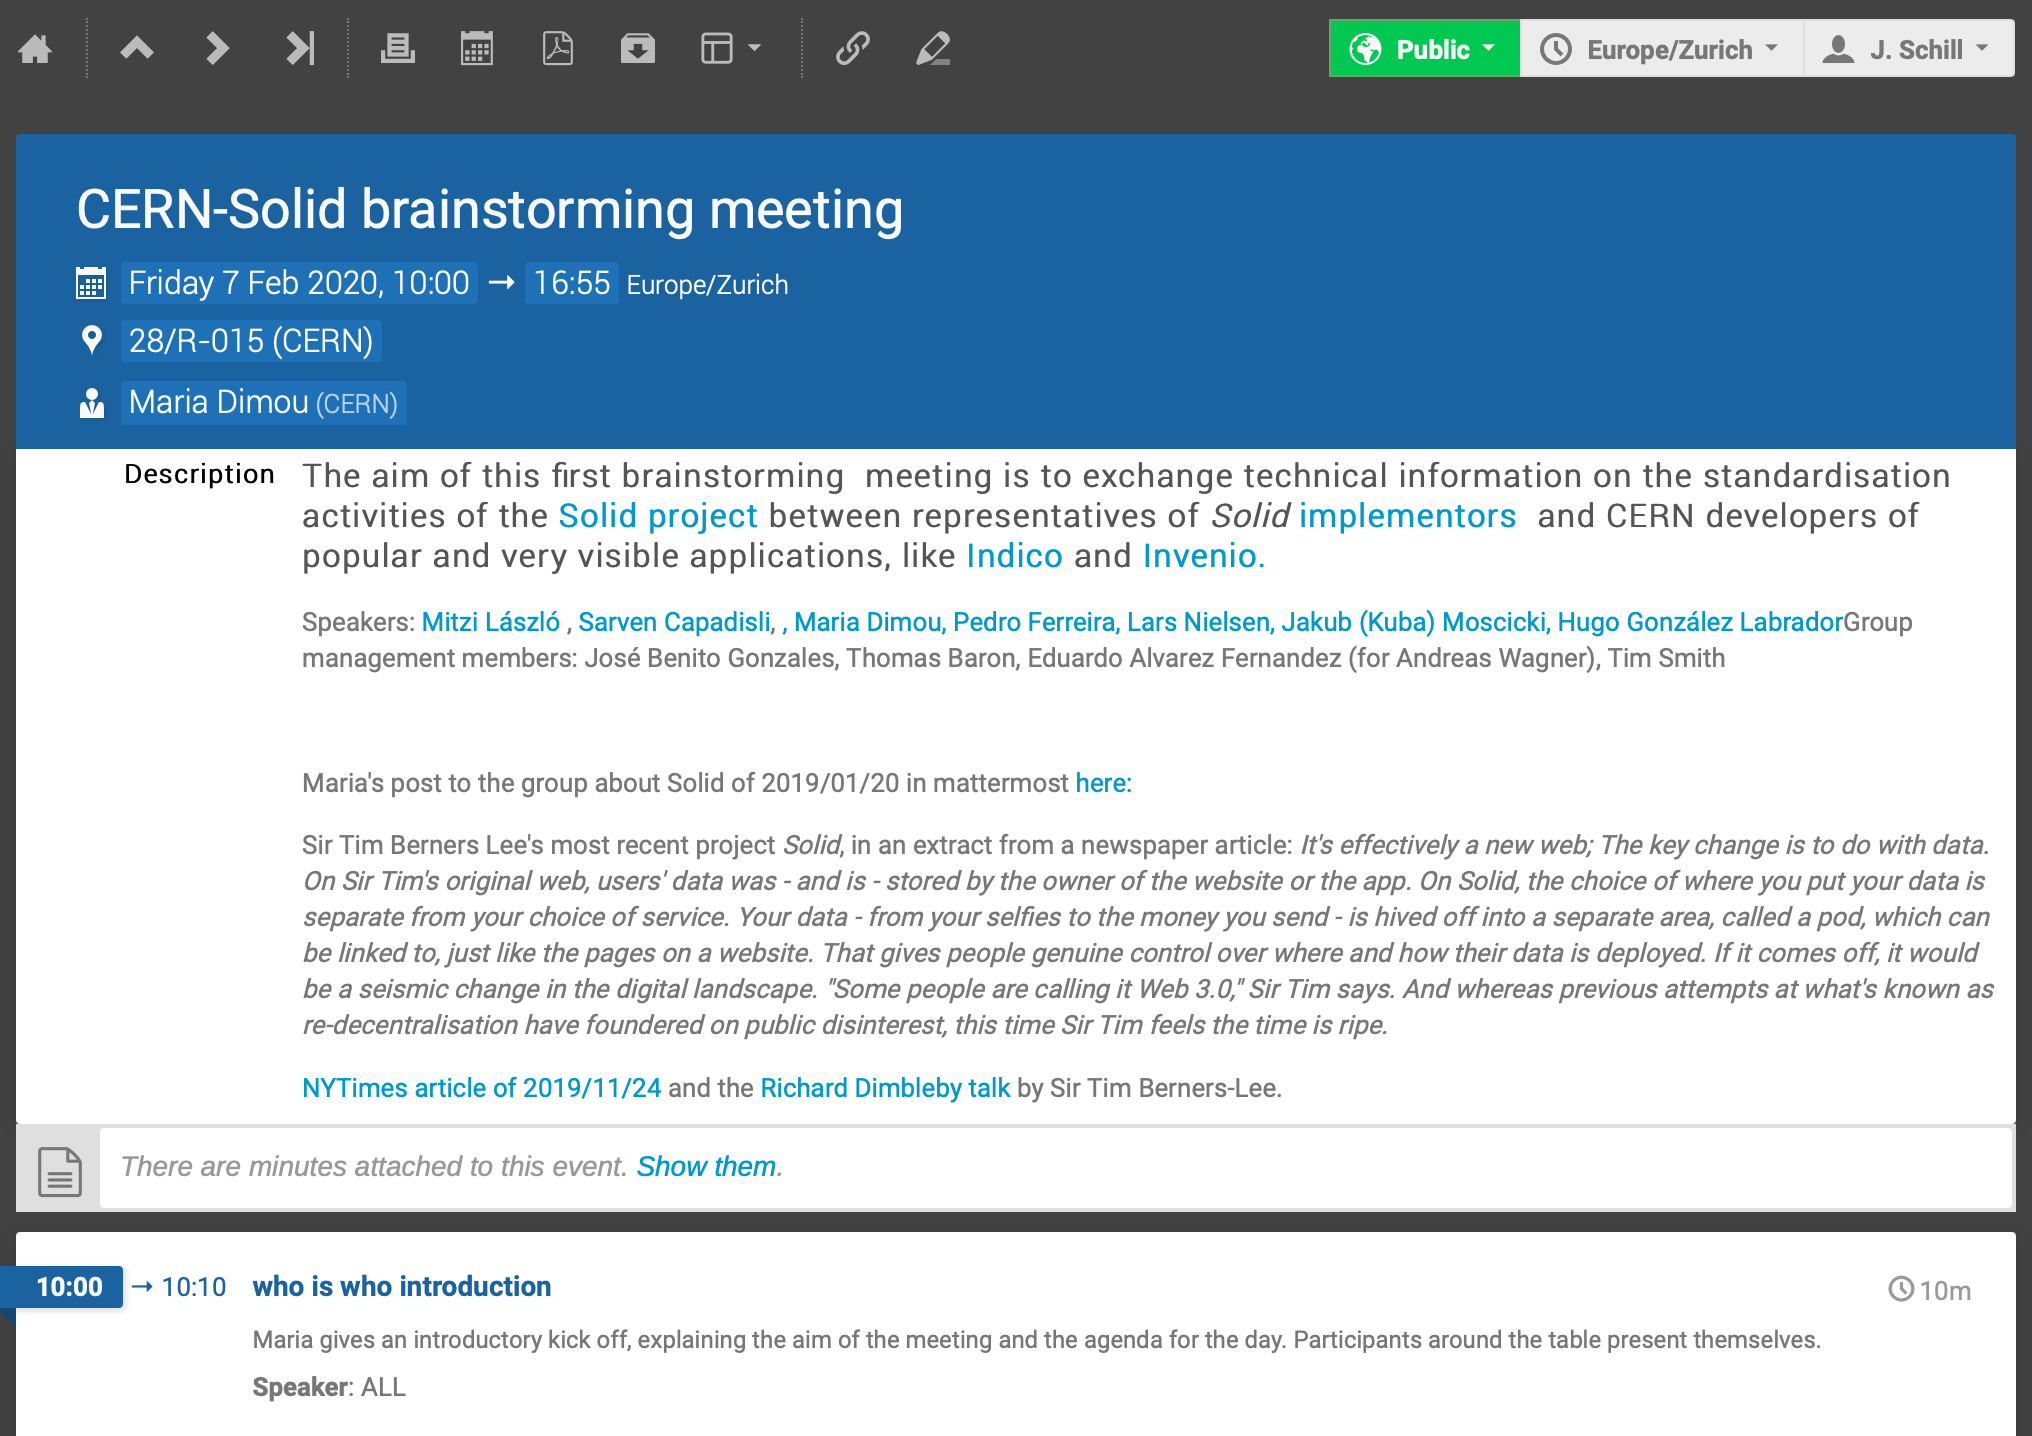
\includegraphics[width=0.6\textwidth]{thesis/latex/assets/indico-event-interface.png}
    \caption{User interface of an Indico event.}
    \label{fig:indico-event-interface}
\end{figure} 

\subsection{Storage Mechanisms}

\subsubsection{EventSettingsProxy}

\subsection{Conference Registration}

\section{Solid}

A prior introduction to Solid was given as part of a previous \textit{research project} \cite{cern-solid-investigation-spec} in preparation to this thesis. In the \textit{research project} the Solid specification was among other things summarized and analyzed. This section will reiterate and study the to the subsequent experiment relevant parts further.

\subsection{Authentication With Solid}

In the Solid ecosystem agents identify themselves with their WebID and proof their ownership through the \gls{solidoidc}, which is a flavor of the \gls{oidc}. For further explanation and flow diagrams throught the authentication process see either the work done in the previous report \cite{cern-solid-investigation-spec} or the \gls{solidoidc} specification itself \cite{solid-ecosystem-oidc}

\subsection{Reading and Writing Linked Data}

\subsection{Authorization Through WAC}

\subsection{Application Launcher}
